%!Tex Program = xelatex
\documentclass[a4paper]{ctexart} % 使用 ctexart 支持中文
\usepackage{amsmath} % 数学公式支持
\usepackage{amsfonts} % 数学符号支持
\usepackage{amssymb} % 数学符号支持
\usepackage{graphicx} % 图片支持
\usepackage{subcaption} % 子图支持
\usepackage{fontspec} % 字体支持
\usepackage{listings}
\usepackage{xcolor}
\lstset{
    backgroundcolor=\color{gray!10},
    frame=single,
    rulecolor=\color{black!30},
    keywordstyle=\color{blue},
    commentstyle=\color{green!50!black}
}
% 定义拉普拉斯算子
\newcommand{\laplace}{\ensuremath{\Delta}}

% 文档信息
\title{Project3 Story}
\author{王方宸 \\ 学号：3210105371}
\date{2024年5月10日}

\begin{document}
\maketitle

\pagestyle{empty}

\section{问题描述}
考虑如下初值问题：
\begin{equation*}
\begin{cases}
    \dot{u}_1 = u_4 \\
    \dot{u}_2 = u_5 \\ 
    \dot{u}_3 = u_6 \\
    \dot{u}_4 = 2u_5 + u_1 - \frac{\mu(u_1+\mu-1)}{r_1^3} - \frac{(1-\mu)(u_1+\mu)}{r_2^3} \\
    \dot{u}_5 = -2u_4 + u_2 - \frac{\mu u_2}{r_1^3} - \frac{(1-\mu)u_2}{r_2^3} \\
    \dot{u}_6 = -\frac{\mu u_3}{r_1^3} - \frac{(1-\mu)u_3}{r_2^3}
\end{cases}
\end{equation*}
其中：
\begin{align*}
    r_1 &= \sqrt{(u_1+\mu-1)^2 + u_2^2 + u_3^2} \\
    r_2 &= \sqrt{(u_1+\mu)^2 + u_2^2 + u_3^2} \\
    \mu &= 0.012277471
\end{align*}

测试案例参数：
\begin{align*}
    \text{模型1: } & \mathbf{u}_0 = (0.994,0,0,0,-2.0015851064,0)^\top,\ T=17.0652165602 \\
    \text{模型2: } & \mathbf{u}_0 = (0.8797792278,0,0,0,-0.3796777809,0)^\top,\ T=19.1405406914
\end{align*}

\section{功能实现}
\subsection{数值功能}
本次项目按要求实现了讲义中要求的线性多步法和单步法：
\begin{itemize}
    \item 单步法
    \begin{itemize}
        \item 经典显式RK方法（Classical RK4）
        \item ESDIRK方法（例11.52，隐式）
        \item Gauss-Legendre RK方法（隐式，$s=2,3,4,5$）
        \item Fehlberg 4(5) 嵌入式RK方法（自适应步长）
        \item Dormand-Prince 5(4) 嵌入式RK方法（自适应步长）
    \end{itemize}
    
    \item 线性多步法
    \begin{itemize}
        \item Adams-Bashforth（显式，$p=1,2,3,4$）
        \item Adams-Moulton（隐式，$p=2,3,4,5$）
        \item BDF（隐式，$p=1,2,3,4$）
    \end{itemize}
\end{itemize}

\subsection{工厂模式}
为实现多种微分方程数值方法的统一管理，采用\textbf{单例模式}封装求解器创建逻辑，核心设计如下：

\begin{itemize}
\item \textbf{单例全局访问}：通过静态方法 \texttt{getInstance()} 获取唯一工厂实例，确保所有求解器注册和创建过程全局一致。
\item \textbf{动态创建接口}：用户通过方法名称和参数（如阶数 $p$）直接创建对应求解器：
\begin{lstlisting}[language=C++, basicstyle=\ttfamily\small]
    // 创建4阶Adams-Bashforth显式求解器
    auto solver = IVPFactory::getInstance()
    .createSolver("AdamsBashforth", 4, T, rhs);
\end{lstlisting}
\end{itemize}

\subsection{项目结构}
我们的核心方法类储存在/src目录下，在/test中是我们的测试与绘图代码，读取/json中的问题模型后，执行$Project3,4$所需的所有测试，以及对未提及比较的ESDIRK方法和Fehlberg 4(5)方法都做了测试，
数据和生成图像分别存放在/data与/plot目录下，对于报告中未体现的部分可以到相应目录进行查看。此外，我们对所有方法均记录了运行时间，储存在/log中。

\section{数值测试以及收敛性}
\subsection{线性多步法}
对于线性多步法，值得说明的一点是隐式方法我们全部采用了不动点迭代法，这在我们的模型中运行良好，但是对于未知模型可能存在隐患，我们设置了不动点迭代最大次数以便于及时提示可能的异常。

我们对两种情况分别进行了测试，要求方法最终计算结果图像与真实情况十分接近。经过测试，我们最后固定所需的迭代次数为：

\subsection*{模型 1}
\begin{table}[h!]
\centering
\begin{tabular}{|c|c|c|c|c|c|}
\hline
\textbf{方法} & $p=1$ & $p=2$ & $p=3$ & $p=4$ & $p=5$ \\ \hline
\textbf{Adams-Bashforth} & 3000000 & 270000 & 60000 & 52000 & / \\ \hline
\textbf{Adams-Moulton} & / & 120000 & 35000 & 25000 & 18000 \\ \hline
\textbf{BDF} & 2500000 & 200000 & 40000 & 28000 & / \\ \hline
\end{tabular}
\caption{模型 1 的迭代次数配置}
\end{table}

\subsection*{模型 2}
\begin{table}[h!]
\centering
\begin{tabular}{|c|c|c|c|c|c|}
\hline
\textbf{方法} & $p=1$ & $p=2$ & $p=3$ & $p=4$ & $p=5$ \\ \hline
\textbf{Adams-Bashforth} & 2000000 & 7000 & 5000 & 1500 & / \\ \hline
\textbf{Adams-Moulton} & / & 5000 & 3000 & 1500 & 800 \\ \hline
\textbf{BDF} & 2500000 & 5000 & 4000 & 1500 & / \\ \hline
\end{tabular}
\caption{模型 2 的迭代次数配置}
\end{table}

下面是一些输出实例，可以看到算法已经与真实解图像相当接近。
\clearpage
\begin{figure}[htbp]
    \centering
    \begin{subfigure}[b]{0.45\textwidth}
        \centering
        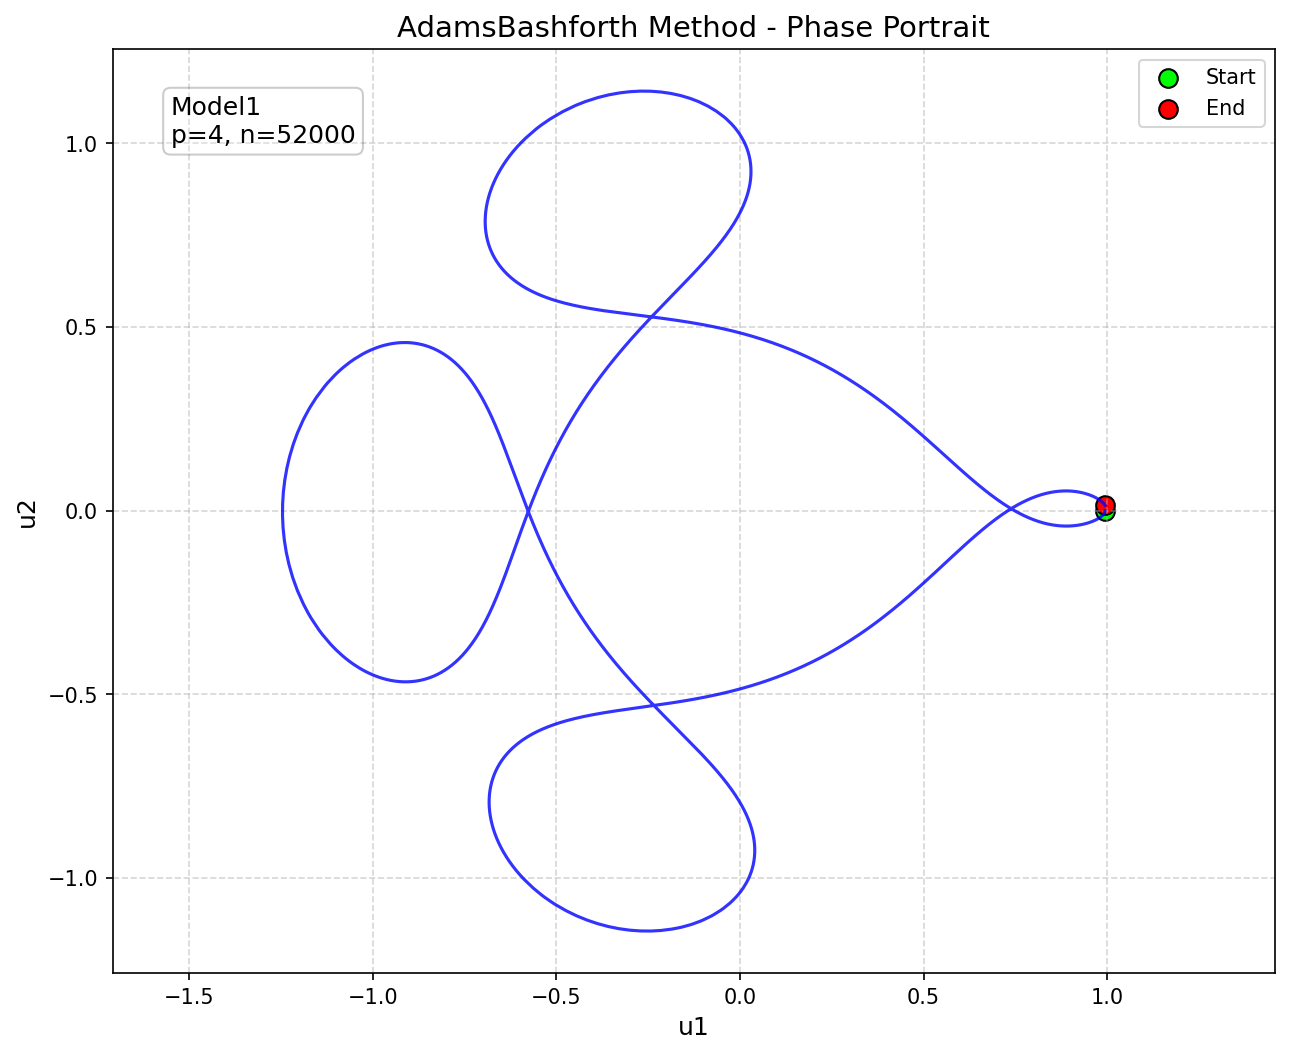
\includegraphics[width=\textwidth]{../plot/AdamsBashforth/Model1_AdamsBashforth_p4_n52000.png}
        \caption{$Model1,AdamsBashforth,p=4,n=52000$}
    \end{subfigure}
    \hfill
    \begin{subfigure}[b]{0.45\textwidth}
        \centering
        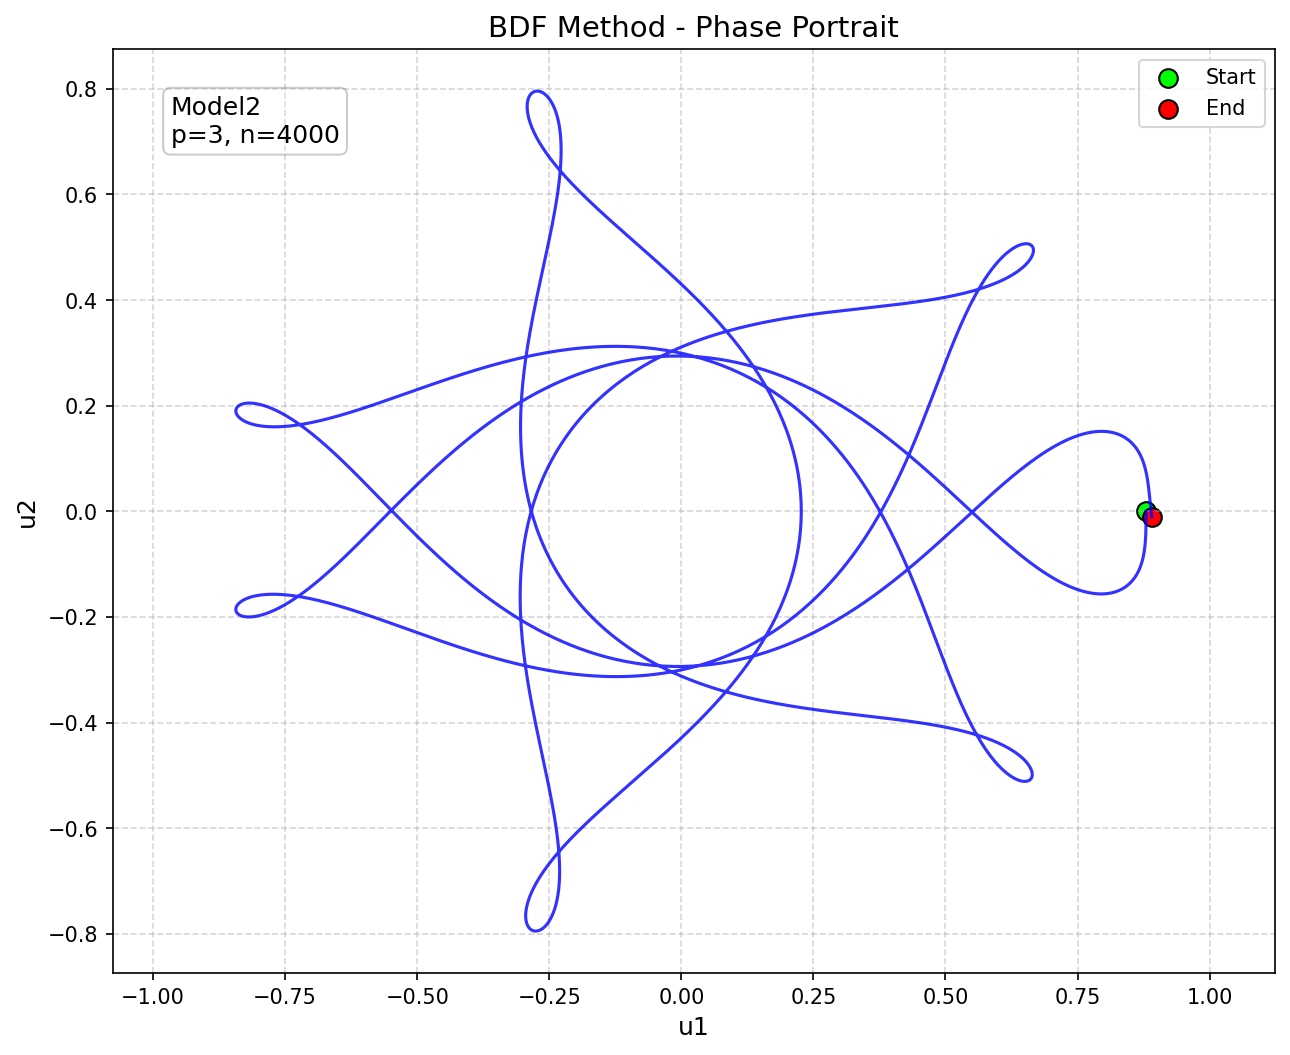
\includegraphics[width=\textwidth]{../plot/BDF/Model2_BDF_p3_n4000.png}
        \caption{$Model2,BDFMethod,p=3,n=4000$}
    \end{subfigure}
    \caption{输出实例}
\end{figure}

\begin{figure}[htbp]
    \centering
    \begin{subfigure}[b]{0.45\textwidth}
        \centering
        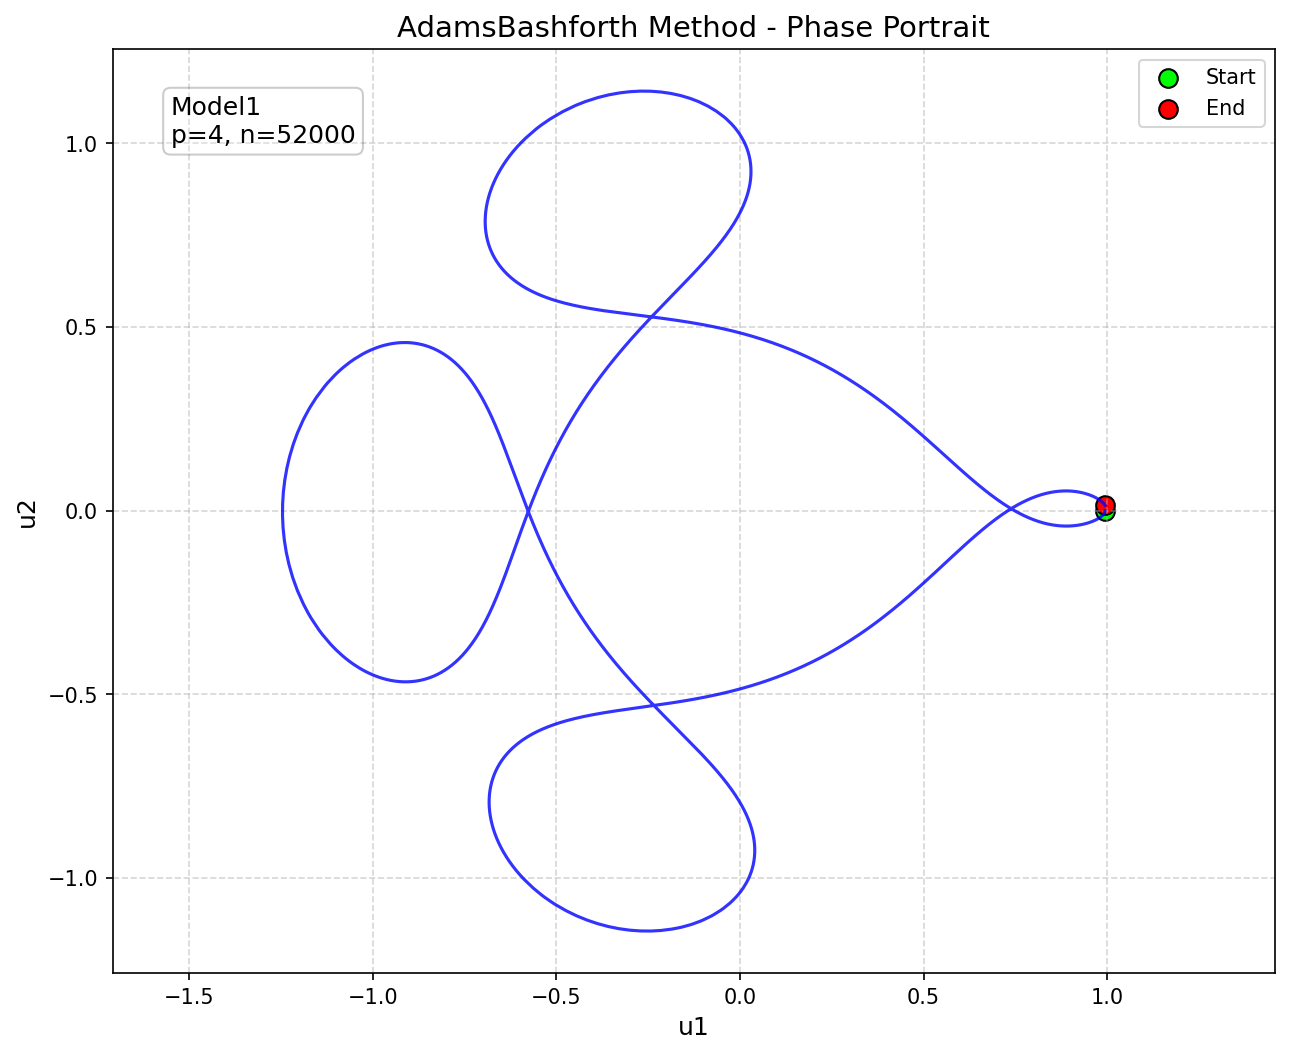
\includegraphics[width=\textwidth]{../plot/AdamsBashforth/Model1_AdamsBashforth_p4_n52000.png}
        \caption{$Model1,AdamsBashforth,p=4,n=52000$}
    \end{subfigure}
    \hfill
    \begin{subfigure}[b]{0.45\textwidth}
        \centering
        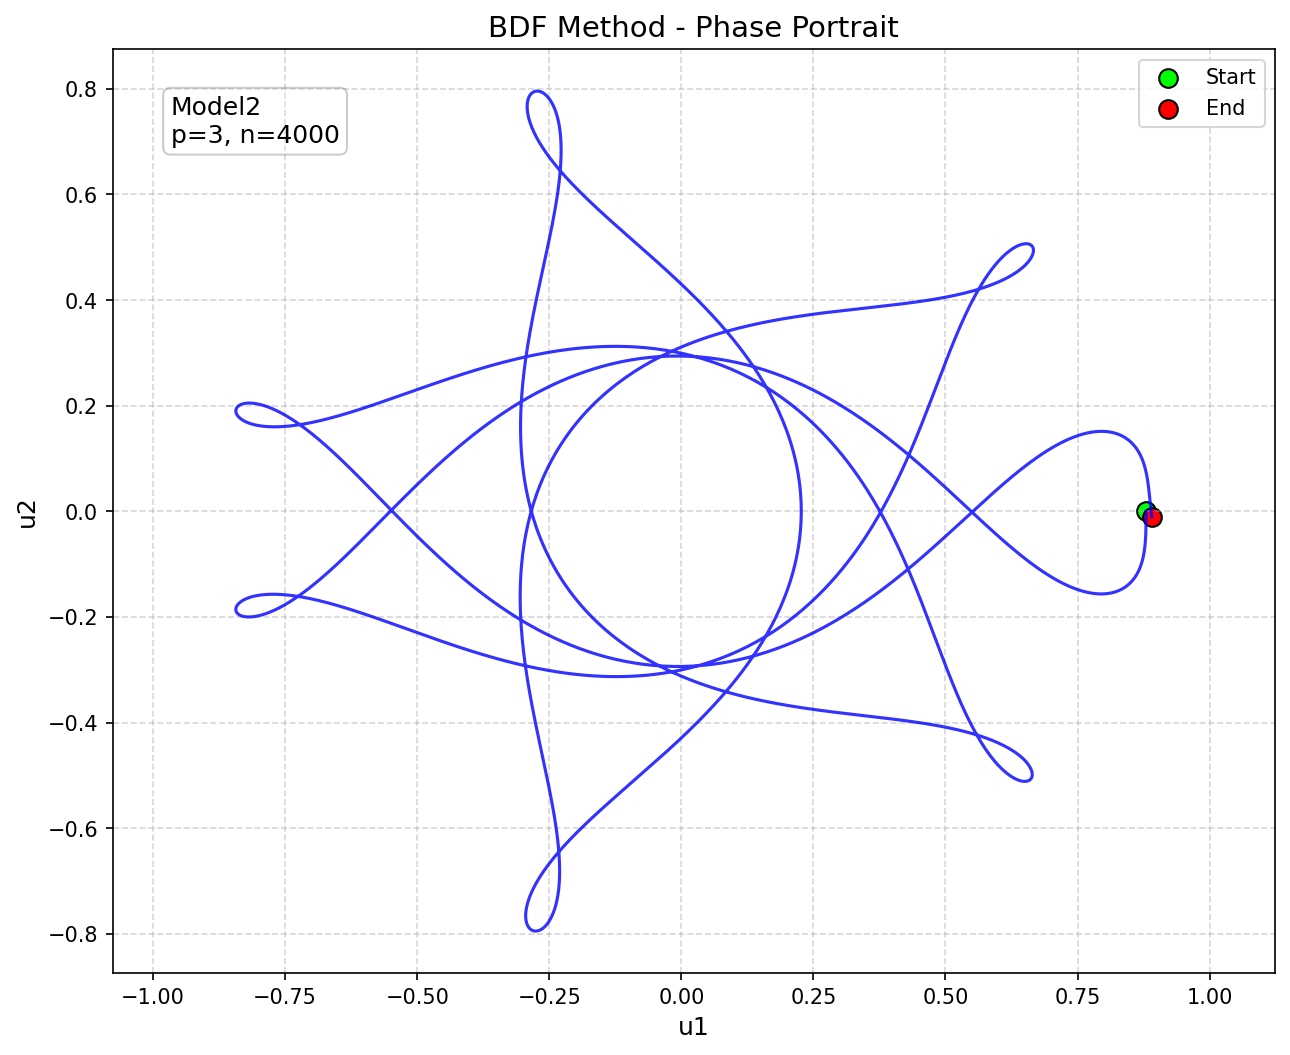
\includegraphics[width=\textwidth]{../plot/BDF/Model2_BDF_p3_n4000.png}
        \caption{$Model2,BDFMethod,p=3,n=4000$}
    \end{subfigure}
    \caption{输出实例}
\end{figure}
\clearpage

\subsection{RK 方法}
对于讲义中的问题，我们分别对以下方法进行了测试：
\begin{itemize}
    \item 欧拉法（Euler method），步数为 24000，固定步长。
    \item 经典的 Runge-Kutta 方法（Classical RK4），步数为 6000，固定步长。
    \item Dormand-Prince 5(4) 嵌套法（Dormand-Prince 5(4) embedded RK method），步数约为 100，自适应步长。
\end{itemize}

运行时间如下：

\begin{table}[h!]
\centering
\begin{tabular}{|c|c|c|c|}
\hline
\textbf{模型} & \textbf{算法} & \textbf{步数} & \textbf{运行时间} \\ \hline
Model 1 & Euler & 24000 & 0.022049 s \\ \hline
Model 1 & Classical RK4 & 6000 & 0.0174912 s \\ \hline
Model 1 & Dormand-Prince 5(4) & (自适应) & 0.0012215 s \\ \hline
Model 2 & Euler & 24000 & 0.0211037 s \\ \hline
Model 2 & Classical RK4 & 6000 & 0.0166145 s \\ \hline
Model 2 & Dormand-Prince 5(4) & (自适应) & 0.0019442 s \\ \hline
\end{tabular}
\caption{RK 方法的运行时间}
\end{table}
下面按顺序给出三种方法的结果图像：
\begin{figure}[htbp]
    \centering
    \begin{subfigure}[b]{0.45\textwidth}
        \centering
        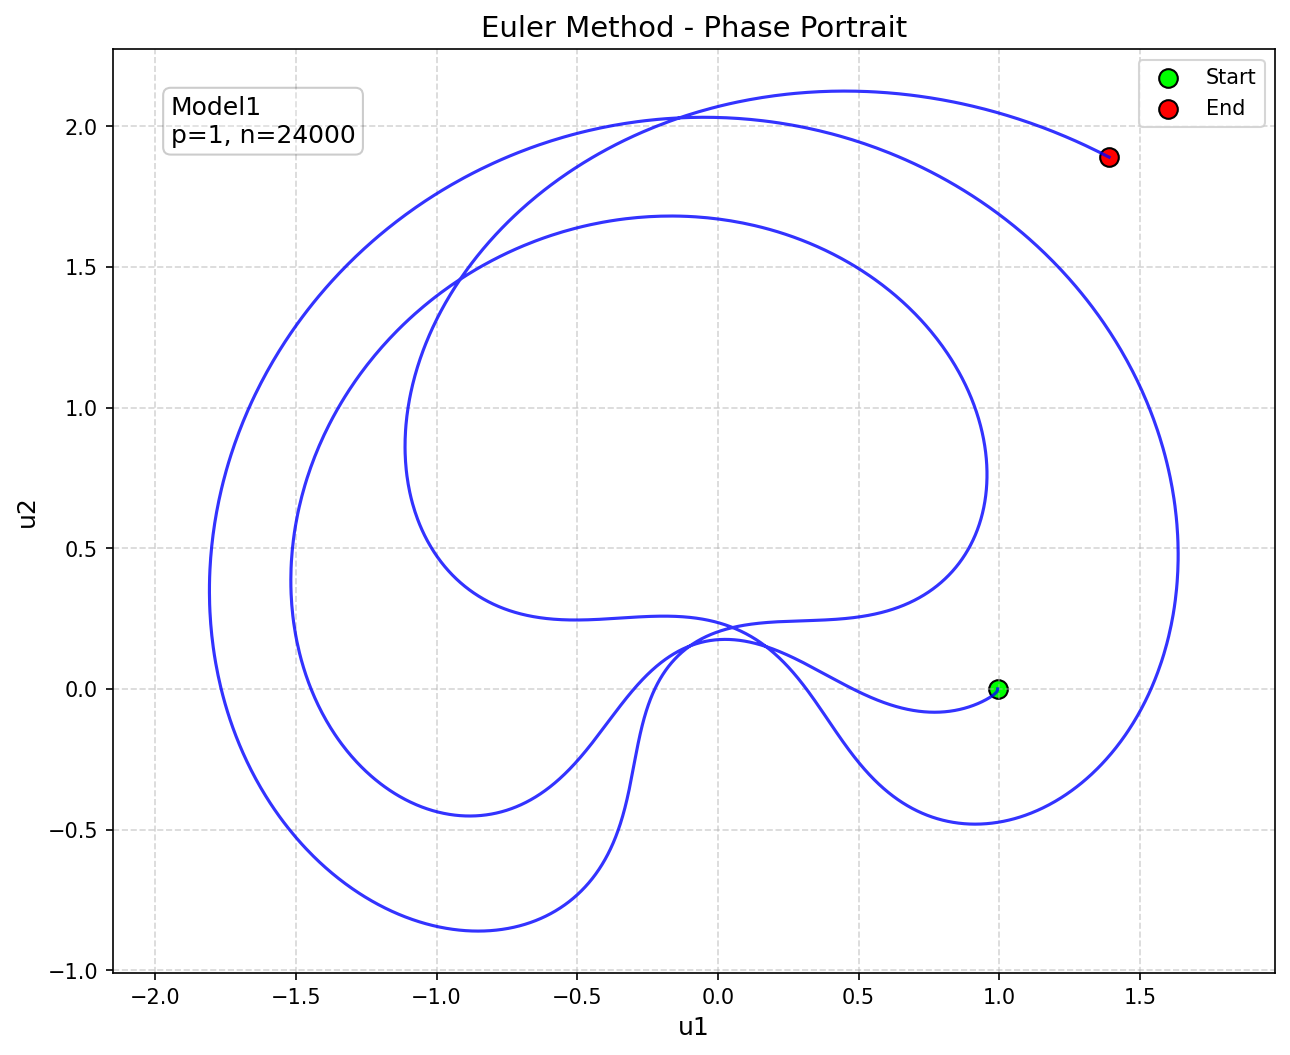
\includegraphics[width=\textwidth]{../plot/Euler/Model1_Euler_p1_n24000.png}
        \caption{$Model1,Euler$}
    \end{subfigure}
    \hfill
    \begin{subfigure}[b]{0.45\textwidth}
        \centering
        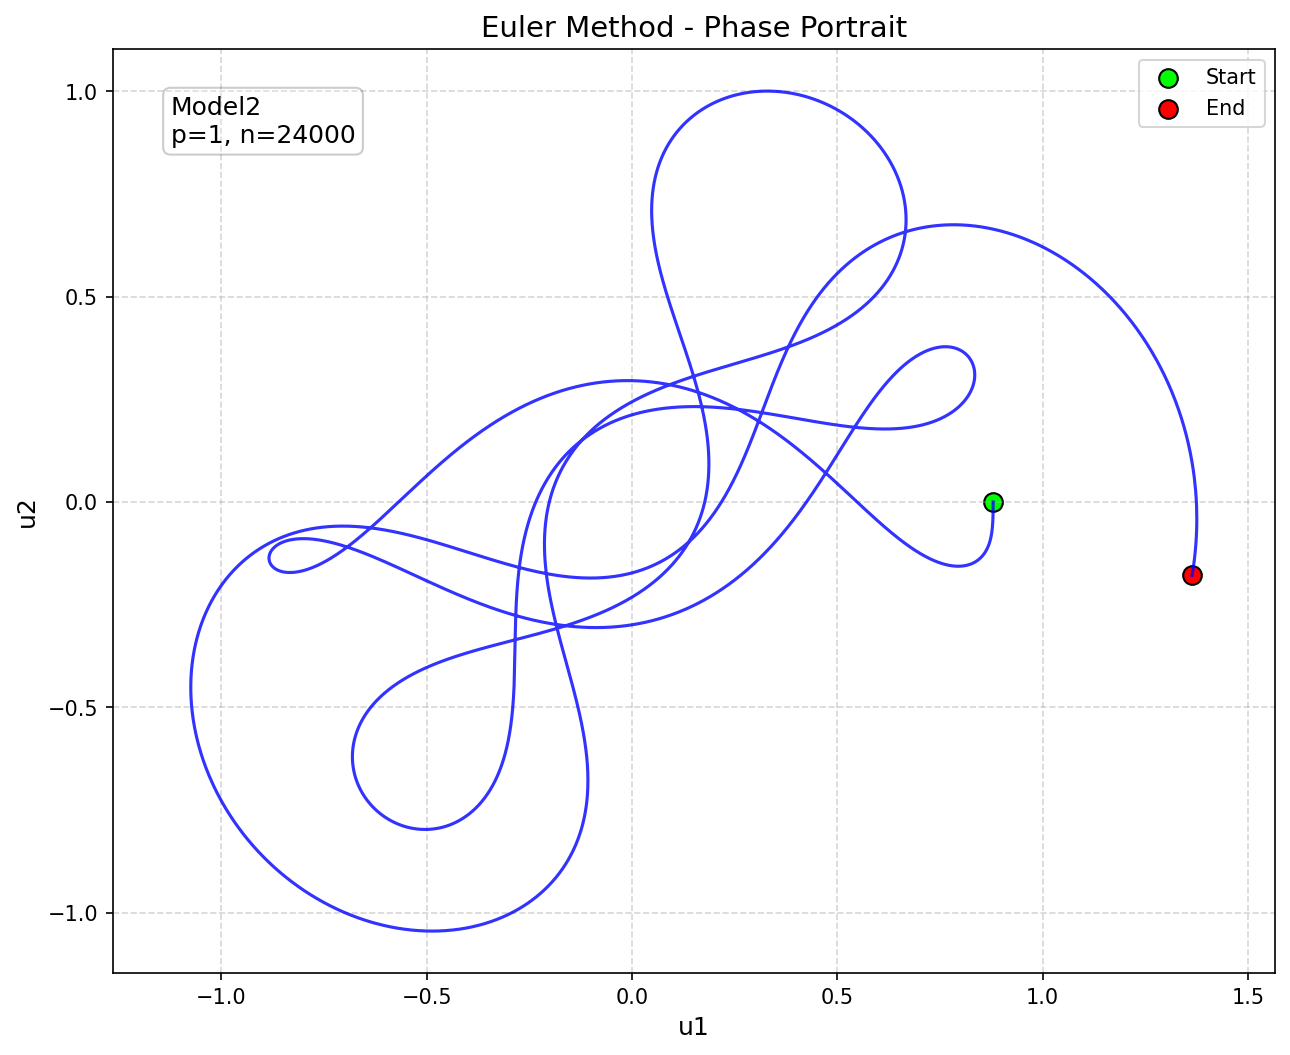
\includegraphics[width=\textwidth]{../plot/Euler/Model2_Euler_p1_n24000.png}
        \caption{$Model2,Euler$}
    \end{subfigure}
    \caption{Euler}
\end{figure}
\clearpage

\begin{figure}[htbp]
    \centering
    \begin{subfigure}[b]{0.45\textwidth}
        \centering
        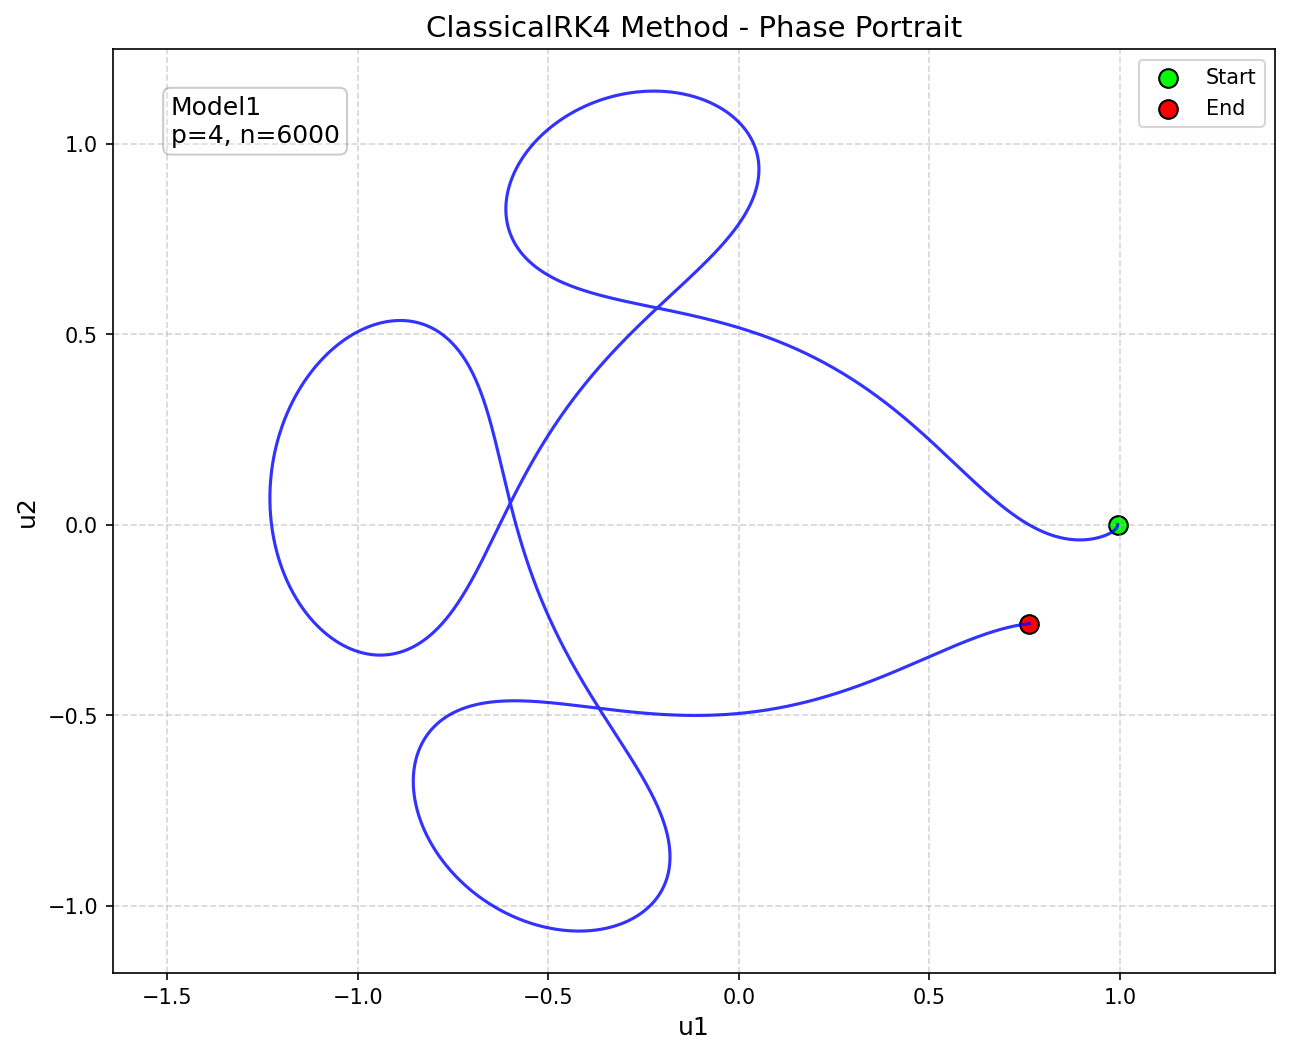
\includegraphics[width=\textwidth]{../plot/ClassicalRK4/Model1_ClassicalRK4_p4_n6000.png}
        \caption{$Model1,ClassicalRK4$}
    \end{subfigure}
    \hfill
    \begin{subfigure}[b]{0.45\textwidth}
        \centering
        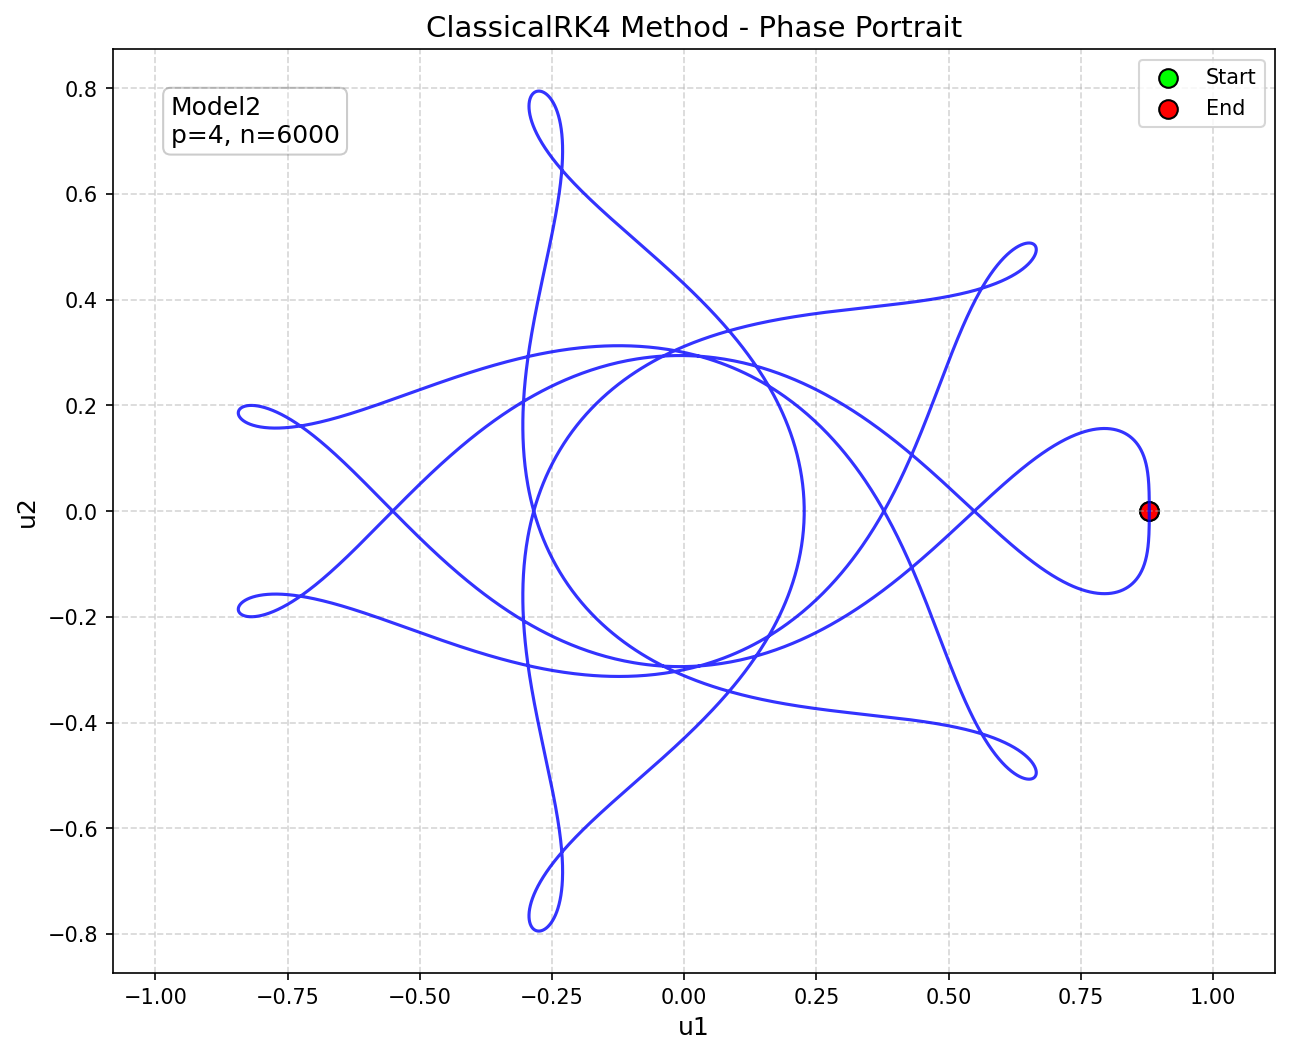
\includegraphics[width=\textwidth]{../plot/ClassicalRK4/Model2_ClassicalRK4_p4_n6000.png}
        \caption{$Model2,ClassicalRK4$}
    \end{subfigure}
    \caption{ClassicalRK4}
\end{figure}

\begin{figure}[htbp]
    \centering
    \begin{subfigure}[b]{0.45\textwidth}
        \centering
        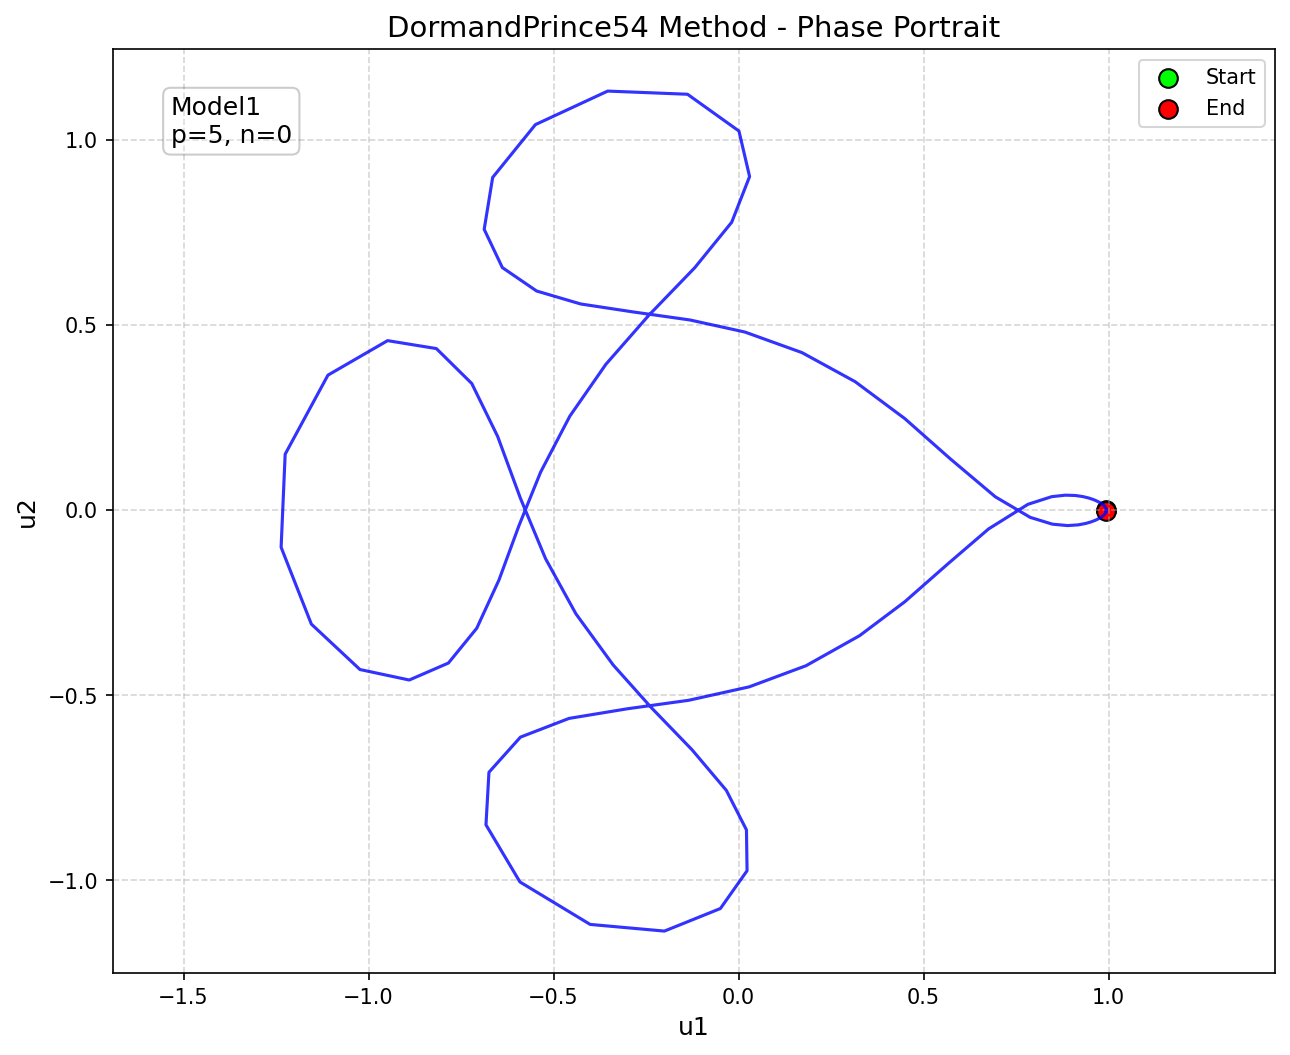
\includegraphics[width=\textwidth]{../plot/DormandPrince54/Model1_DormandPrince54_p5_n0.png}
        \caption{$Model1,DormandPrince54$}
    \end{subfigure}
    \hfill
    \begin{subfigure}[b]{0.45\textwidth}
        \centering
        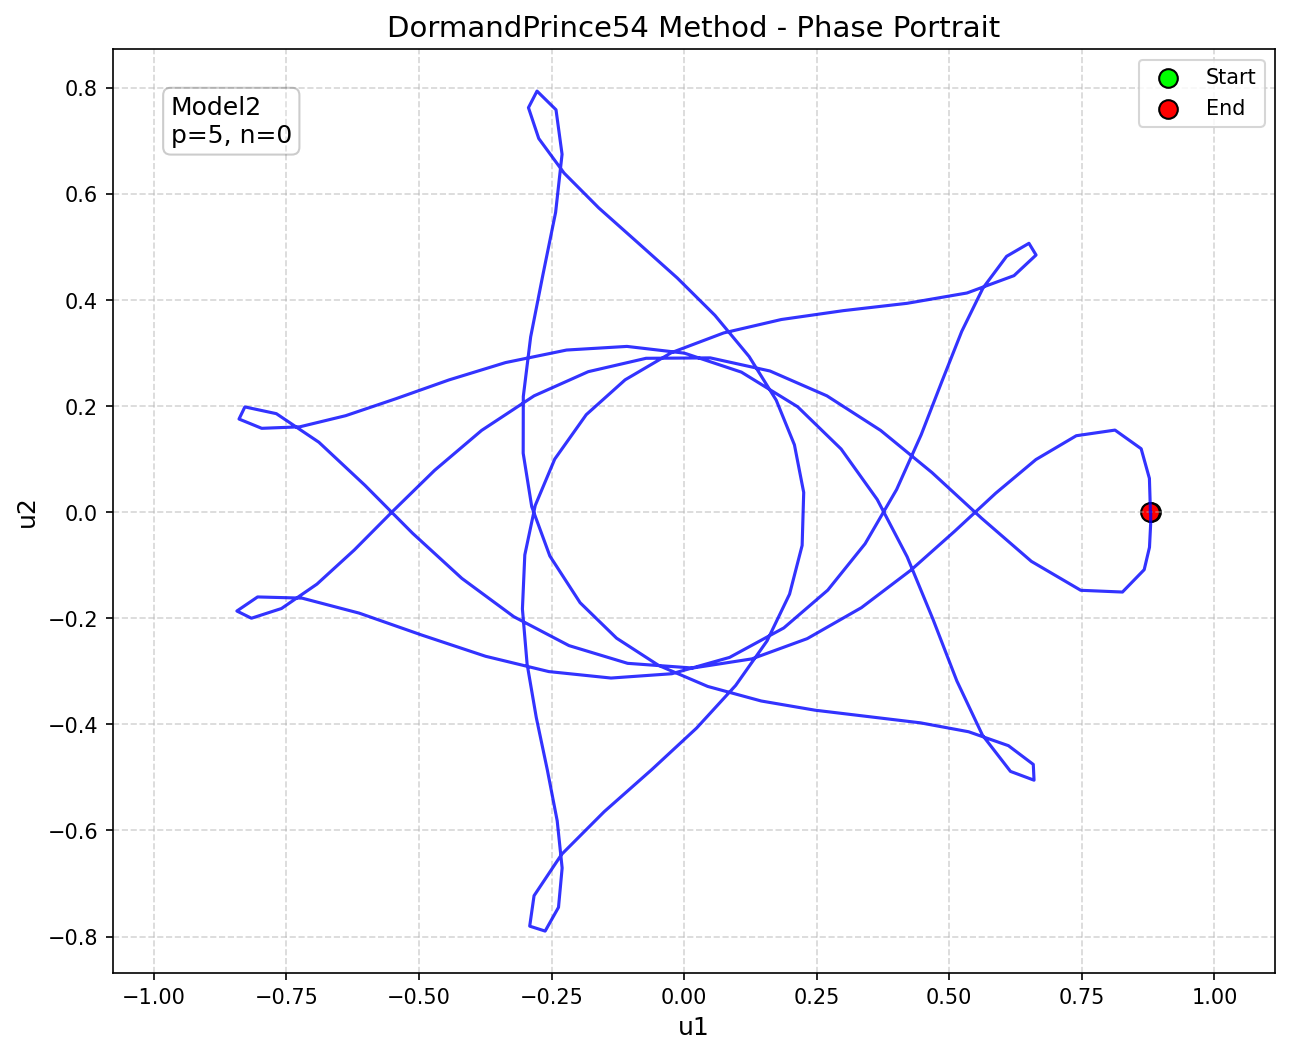
\includegraphics[width=\textwidth]{../plot/DormandPrince54/Model2_DormandPrince54_p5_n0.png}
        \caption{$Model2,DormandPrince54$}
    \end{subfigure}
    \caption{DormandPrince54}
\end{figure}
可以看到Euler方法的图像几乎还没有收敛，而经典RK法基本收敛，Dormand-Prince 5(4)虽然格点数目少，但是图像已经很精准。

同时，从运算时长来说，Dormand-Prince 5(4)方法所需的时间也最短，比Euler和经典RK算法快一个数量级，这体现了Dormand-Prince 5(4)方法的优越性。
\clearpage

此外，我们还对未在问题中出现的ESDIRK（为测试运行效率选取最高阶）和Fehlberg 4(5)方法进行了测试，可以看到算法运行良好，验证了代码的准确性。
\begin{figure}[htbp]
    \centering
    \begin{subfigure}[b]{0.45\textwidth}
        \centering
        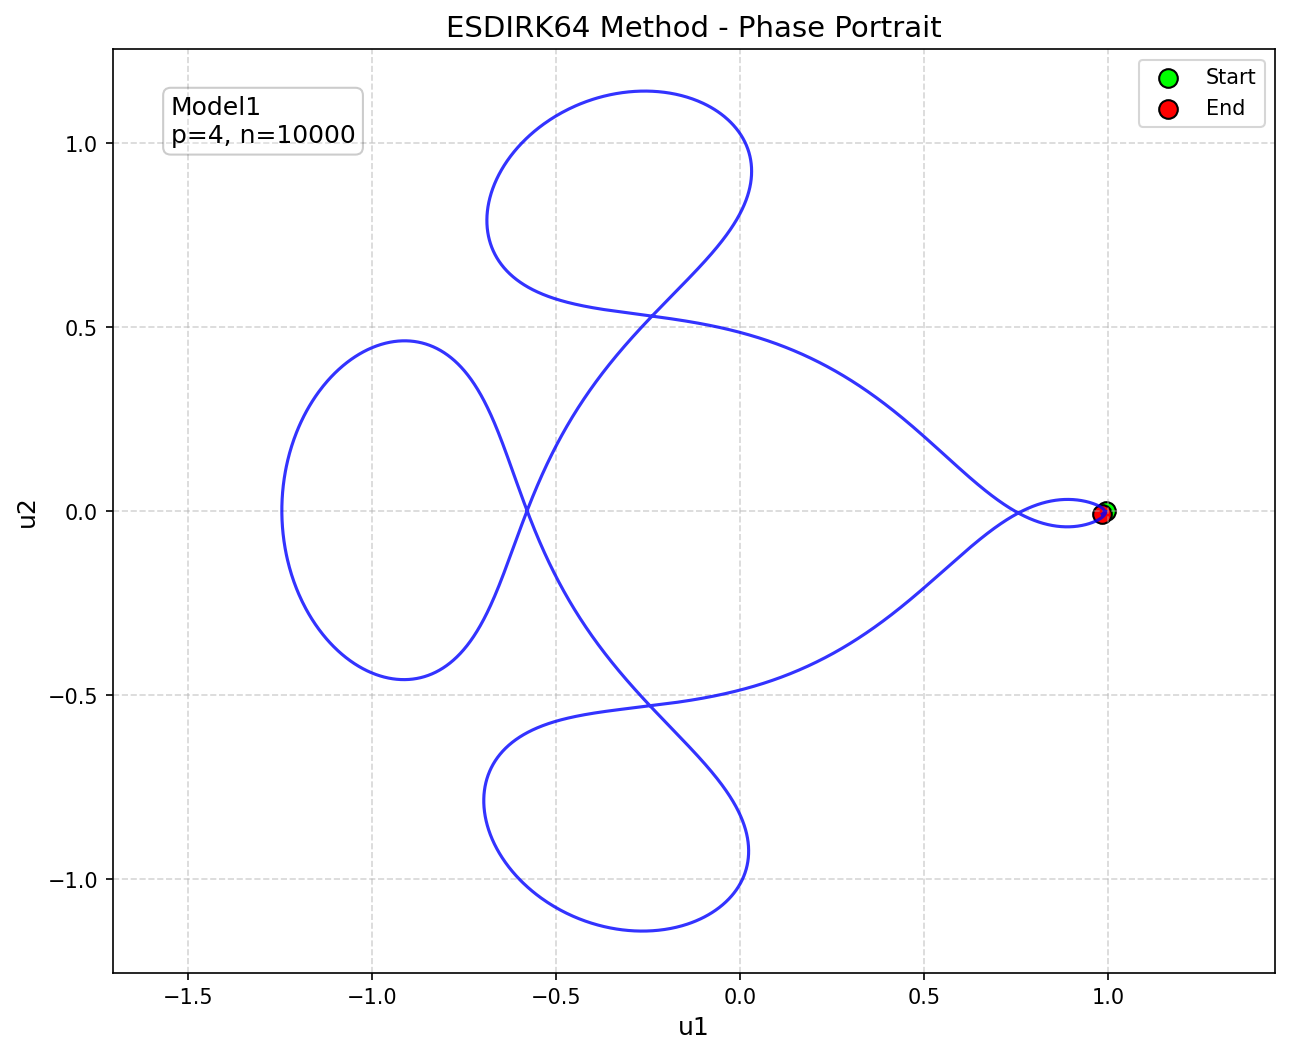
\includegraphics[width=\textwidth]{../plot/ESDIRK64/Model1_ESDIRK64_p4_n10000.png}
        \caption{$Model1,ESDIRK,p=4,n=10000$}
    \end{subfigure}
    \hfill
    \begin{subfigure}[b]{0.45\textwidth}
        \centering
        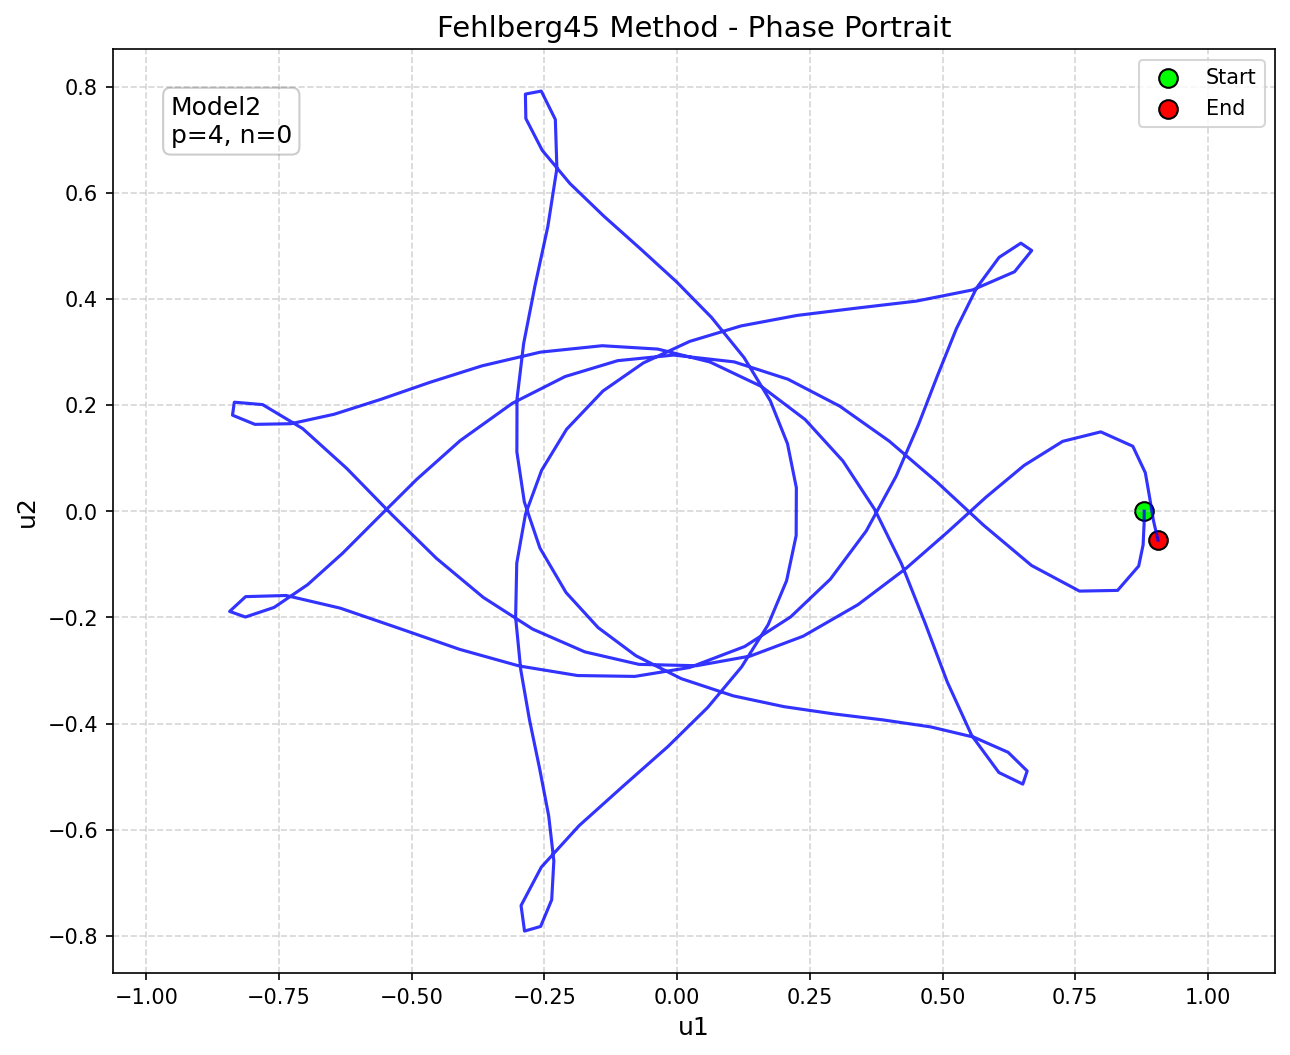
\includegraphics[width=\textwidth]{../plot/Fehlberg45/Model2_Fehlberg45_p4_n0.png}
        \caption{$Model2,Fehlberg45$}
    \end{subfigure}
    \caption{}
\end{figure}

\subsection{对线性多步法的收敛性测试}
本次项目对线性多步法也进行了收敛阶的测试，我们选取了上述模型 1，设置 $N = 100000$，由于问题模型的周期性，
对 $N, 2N, 4N$ 的迭代步长分别计算其首尾的误差，然后计算阶数。

收敛阶分析结果如下：
\clearpage

\begin{table}[h!]
\centering
\begin{tabular}{|c|c|c|c|}
\hline
\textbf{方法} & \textbf{$p$} & \textbf{观测阶数} & \textbf{理论阶数} \\ \hline
Adams-Bashforth & 1 & 0.05 & 1 \\ \hline
Adams-Bashforth & 2 & 0.39 & 2 \\ \hline
Adams-Bashforth & 3 & 2.75 & 3 \\ \hline
Adams-Bashforth & 4 & 3.86 & 4 \\ \hline
Adams-Moulton & 2 & 1.27 & 2 \\ \hline
Adams-Moulton & 3 & 2.79 & 3 \\ \hline
Adams-Moulton & 4 & 3.95 & 4 \\ \hline
Adams-Moulton & 5 & 6.19 & 5 \\ \hline
BDF & 1 & 0.01 & 1 \\ \hline
BDF & 2 & 0.63 & 2 \\ \hline
BDF & 3 & 2.47 & 3 \\ \hline
BDF & 4 & 3.92 & 4 \\ \hline
\end{tabular}
\caption{线性多步法的收敛阶分析结果}
\end{table}

在阶数较低时，可能我们选取的 $N$ 的表现对于此时的整体表现较差（但是为了整体项目的测试速度，我们这里没有区分开做）。而对于相对较高的阶数，可以看到我们的收敛阶基本符合理论预期。


\end{document}
